\documentclass[10pt, a4paper,openany]{article}
\usepackage[italian]{babel}
\usepackage[T1]{fontenc}
\usepackage[table]{xcolor}
\usepackage{float}
\restylefloat{table,figure}
\usepackage{graphicx}	
\usepackage[utf8]{inputenc}
\usepackage{amsmath}
\usepackage{fancyhdr}
\usepackage{geometry}
\usepackage{url}
\usepackage{hyperref}
\usepackage[ruled,vlined]{algorithm2e}
\geometry{a4paper,top=2cm,bottom=2cm,left=3cm,right=3cm,%
	heightrounded,bindingoffset=5mm}
\usepackage{amssymb}
\usepackage{amsthm}


\begin{document}

\begin{center}
\huge\textbf{YouTube al tempo del Covid-19}

Un'analisi dei video in tendenza
\end{center}

\begin{center}
Gabriele Celeri, Federico Luzzi,  Marco Peracchi, Christian Uccheddu
\end{center}

\hrule
\vspace{0.2cm}
\begin{center}\textbf{Introduzione e obiettivi}\end{center} 
Negli ultimi mesi il Covid-19 ha avuto un impatto notevole sulle vite di tutti noi. L'obiettivo di questo lavoro è capire se la piattaforma YouTube sia stata influenzata dalla presenza di questo virus che ha costretto a rimanere nelle proprie case gran parte della popolazione mondiale. 
Per valutare l'impatto della pandemia e della quarantena obbligatoria, abbiamo confrontato i video in tendenza di Youtube nel periodo Dicembre-Gennaio rispetto Marzo-Maggio, con l'obiettivo di verificare se i contenuti presenti sulla piattaforma e la loro tipologia siano cambiati.
Inoltre, ci siamo preposti, come secondo obiettivo, di verificare se l'andamento dei contagi, e delle notizie in merito, specialmente se negative, influenzassero in alcun modo la fruizione di video riguardanti il Covid-19.
\\\\ \begin{small}
	\textit{Keyword: Covid-19, YouTube}
\end{small}
\vspace{0.2cm}
\hrule

\subsection*{Scelta degli strumenti (DA RISCRIVERE)}
La prima domanda che ci siamo posti riguardo al progetto è stata: "Quali sono le "V" su cui focalizzare la nostra attenzione?".
Dopo qualche indagine preliminare abbiamo deciso che che ci saremmo concentrati su "Volume" e su "Velocity", perché i nostri dati venivano raccolti in tempo reale dalle API di Youtube e la quantità di dati aumenta costantemente con l'aumentare del tempo di presa dati.

Per gestire il flusso di dati ci siamo affidati al software Kafka, permettendoci così di poter disaccoppiare la fase di lettura dei dati dalla fase di  raccolta. Uno script python (\textit{scraper\_producer.py}) si occupava del producer, continuando ad effettuare richieste alle API di youtube, mentre lo script consumer (\textit{scraper\_consumer.py}) si occupava di leggere i file memorizzati nel topic di kafka, e successivamente di immagazzinarli in un database MongoDB in formato JSON. La scelta di MongoDB è stata dettata dalla sorgente dei dati, che venivano forniti in formato documentale.
\section*{Raccolta dati}
La raccolta dati è basata su due fonti principali: YouTube e [fonte/i covid-19].
\subsection*{Youtube API}
I video in tendenza su youtube variano ogni 15 minuti circa (fonte: \url{https://support.google.com/youtube/answer/7239739?hl=it}) anche se non per forza e solitamente vi è solo una manciata di video che entra/esce dalle tendenze. Per la raccolta di questi dati ci siamo basati sulle funzioni API messe a disposizione da youtube per poter raccogliere i video in tendenza in un dato momento. Le chiavi di richiesta gratuite fornite da Google developer però ci permettono di effettuare una quantità limitata di richieste. 
\\
Abbiamo effettuato sostanzialmente due differenti \textbf{sessioni} di scraping, con metodi leggermente differenti, dovuti allo scopo che ci eravamo prefissati: 
\begin{enumerate}
	\item dal 23 dicembre 2019 al 5 gennaio 2020 (raccolta ogni 30 minuti)
	\item dal 18 marzo 2020 al 6 maggio 2020 (raccolta ogni 6 ore)
\end{enumerate}
Abbiamo deciso di raccogliere dati delle tendenze dei seguenti paesi:

Italia, USA, Regno Unito, India, Germania, Canada, Francia, Corea del sud, Russia, Giappone, Brasile, Messico\\

\subsection*{Prima sessione}
Inizialmente pensavamo di utilizzare i dati per analizzare come, in generale, un video riesce ad arrivare nelle tendenze di youtube e in base a questo fatto analizzare il suo comportamento per quanto riguarda visualizzazioni, likes, dislikes, ecc. La raccolta in questa sessione viene effettuata con lo script \textit{scraper\_timed.py} che sostanzialmente esegue questi passaggi:\\
\\
\begin{algorithm}[H]
	\KwData{country - insieme dei paesi prescelti; videos - insieme di video scaricati da un determinato paese}
	\nl \For{every 30 minutes} {
	\nl \ForEach{country}
	{
		\nl videos = APIrequest(max(50 video), country)\\
		\nl \While {video in tendenza non finiti}
		{
			\nl videos += APIrequest(max(50 video), country) \\
		}
		\nl videos\_fix = arrangeData(videos)\\ 
		\nl saveToCsv(videos\_fix) \\
		\nl videos = $\emptyset$
	}
	}
	\caption{Scraping youtube $\rightarrow$ csv}
\end{algorithm}

%Alternativa per scrivere l'algoritmo
%\begin{enumerate}
%	\item Per ogni paese prescelto
%	\item API request sulle tendenze del momento $\rightarrow$ download di page da 50 video [formato json]
%	\item ripeti 2. finchè scarica tutti i video
%	\item copio le informazioni formattate in formato csv (vedi dopo) 
%	\item ripeti da 2. per ogni paese
%	\item attendi 30 minuti (scheduler)
%	\item ripeti da 1.
%\end{enumerate}
\underline{Nota}: per ogni API request al massimo possiamo scaricare 50 video e ogni paese a un numero diverso di video in tendenza (solitamente 150-200).

In questa sessione abbiamo pensato di salvare i dati in formato \textit{csv}
modo tale che siano facilmente manipolabili. Segue lo schema logico con cui li abbiamo immagazzinati:
\begin{table}[H]
	\centering
	\begin{tabular}{l|l}
		\textbf{Attributo} & \textbf{Descrizione} \\
		\hline
		\textbf{timestamp} & data, ora e minuto della nostra rilevazione \\\hline
		\textbf{video\_id} & identificativo unico del video\\\hline
		\textbf{title} & nome del video per esteso\\\hline
		\textbf{publishedAt} & data di pubblicazione\\\hline
		\textbf{channelId} & identificativo unico del canale che ha pubblicato il video\\\hline
		\textbf{channelTitle} & nome del canale per esteso\\\hline
		\textbf{categoryId} & identificativo unico della categoria\\\hline
		\textbf{trending\_date} & data in cui il video è in tendenza\\\hline
		\textbf{tags} & stringa dei tag usati separati dal carattere "|"\\\hline
		\textbf{view\_count} & numero di visualizzazioni\\\hline
		\textbf{likes} & numero di like (mi piace)\\\hline
		\textbf{dislikes} & numero di dislike (non mi piace)\\\hline
		\textbf{comment\_count} & numero di commenti sotto il video\\\hline
		\textbf{thumbnail\_link} & url all'immagine di copertina del video\\\hline
		\textbf{comments\_disabled} & booleano che dichiara se i commenti sono disabilitati\\\hline
		\textbf{ratings\_disabled} & booleano che dichiara se i like/dislike sono disabilitati\\\hline
		\textbf{description} & descrizione del video\\
		\hline
	\end{tabular}
	\caption{schema degli attributi dei dati csv}
\end{table}

I dati così raccolti sono salvati nella cartella [INSERIRE NOME CARTELLA]

\subsection*{Seconda sessione}

Per la seconda sessione di raccolta, in cui abbiamo deciso di concentrarci sugli effetti che l'epidemia del nuovo virus Covid-19, abbiamo adottato un approccio diverso. Innanzitutto abbiamo deciso di immagazzinare i dati in un database mongoDB nativamente. Pertanto oltre a costruire una pipeline di raccolta che salva i dati direttamente su mongoDB abbiamo deciso parallelamente di immagazzinarli in formato \textit{json}. 

Seconda considerazione è stata data la bassa variabilità dei video raccogliendo i dati ogni 30 minuti, vista nella precedente sessione, abbiamo deciso di effettuare lo scraping ogni 6 ore, in modo da avere 4 rilevazioni durante una giornata. 

A scopo didattico abbiamo inoltre deciso di implementare una piccola pipeline Kafka in cui dividiamo la fase di raccolta dati (\textit{scraper\_producer.py}) e la fase di immagazzinamento (\textit{scraper\_consumer.py}). 

\begin{figure}[H]
	\centering
	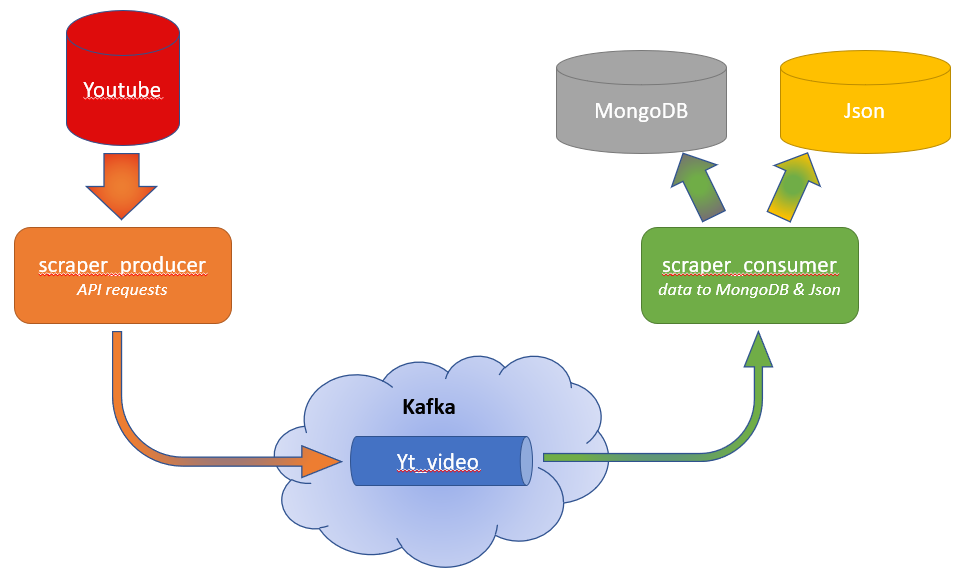
\includegraphics[width=0.8\linewidth]{pics/pipeline.png}
	\caption{pipeline di raccolta dati - seconda sessione}
\end{figure}

Di seguito il dettaglio della computazione dei 2 script:

\begin{algorithm}[H]
	\KwData{country - insieme dei paesi prescelti; videos - insieme di video scaricati da un determinato paese; KafkaProducer(data, channel) - sends data to channel kafka}
	\nl \For{every 6 hours} {
		\nl \ForEach{country}
		{
			\nl videos = APIrequest(max(50 video), country)\\
			\nl KafkaProducer(videos, yt\_video) \\ 
			\nl \While {video in tendenza non finiti}
			{
				\nl videos = APIrequest(max(50 video), country) \\
				\nl KafkaProducer(videos, yt\_video) \\
			}
		}
	}
	\caption{scraper producer}
\end{algorithm}

\begin{algorithm}[H]
	\KwData{KafkaConsumer(channel) - receives data from channel kafka}
	\nl \While{loop} {
		\nl \If{KafkaConsumer(yt\_video) $\ne \emptyset$}
		{
			\nl videos = KafkaConsumer(yt\_video)\\
			\nl videos\_fix = arrangeData(videos)\\ 
			\nl saveToJson(videos\_fix)\\
			\nl saveToMongoDB(videos\_fix)
		}
	}
	\caption{scraper consumer}
\end{algorithm}
I dati così raccolti sono stati salvati in formato json nella cartella [INSERIRE NOME CARTELLA].

\underline{Nota}: abbiamo scelto di salvare i dati in formato Json in modo che fosse facile caricarli in un nuovo server mongoDB e renderli più trasportabili. Per il caricamento vedi lo script: \textit{json\_to\_mongo.py}

Lo schema logico dei documenti json è sostanzialmente lo stesso di quello dei csv visto precedentemente in \textit{Tabella 1} ma con due variazioni:
\begin{itemize}
	\item \textbf{tags} immagazzinati come array di stringhe
	
	Ad esempio:
	
	tags: ["covid-19", "quarantena"]
	\item informazioni relative ai likes, dislikes, view\_count e comment\_count innestati in un oggetto \textbf{statistics}
	
	Ad esempio:
	
	statistics: \{view\_count: 14235,
				likes: 513,
				dislikes: 34,
				comment\_count: 254
				\}
\end{itemize}
\subsection*{Dati Covid-19}
Qua dobbiamo scrivere come/dove abbiamo preso i dati covid

  
\subsection*{Qualità dati}
La grande disponibilità di dati ha rappresentato il problema più rilevante della verifica di qualità. Fortunatamente i dati non presentavano problemi di \textit{missing values} che avrebbero rappresentato difficoltà non trascurabili. Le principali problematiche emerse sono due:
\begin{itemize}
	
	\item Ridondanza: I dati di Dicembre-Gennaio presentano richieste effettuate ai server di Youtube ogni mezz'ora, a differenza del periodo successivo. Di conseguenza sono stati rilevati molti dati simili tra loro, senza alcuna sostanziale variazione nelle varie fasce delle giornata. Per risolvere il problema abbiamo optato per scegliere quattro rilevazioni distaccate di sei ore ciascuna, in maniera da uniformare i dati con quelli di marzo-maggio. Per ulteriori dettagli è possibile visualizzare il notebook jupyter con cui è stato affrontato il problema.

	\item Saturazione richieste: Google non permette di effettuare troppe richieste nella stessa giornata. Per arginare il problema abbiamo utilizzato tre API key differenti da alternare durante la presa dati. Nonostante questo espediente ci sono stati alcuni momenti dove non è stato possibile effettuare le richieste ai server. Come risoluzione di questo problema abbiamo duplicato i dati della richiesta precedente, poiché le tendenze estratte in tempi ravvicinati non presentano variazioni importanti nei video.
	
	
\end{itemize}

\subsection*{Integrazione dati}
	Per poter rispondere alle nostre domande di ricerca abbiamo dovuto effettuare un'integrazione tra i dati dei video di Youtube e i dati relativi alla pandemia da Covid-19. L'integrazione è avvenuta prima del caricamento dei dati su MongoDB, lo script che mostra l'operazione è \textit{merge\_to\_mongo.py}. 
	
	Per ricavare le informazioni relative all'andamento della pandemia nella giornata considerata abbiamo effettuato un'\textbf{integrazione temporale}, dove le chiavi considerate sono state il \textbf{timestamp} e il \textbf{country\_name}, cioè la data e il paese. Il procedimento è il seguente: viene ricercata la data del video considerato e il paese di appartenenza, e successivamente viene creato un dizionario con tutte le informazioni della pandemia nella data e paese appena cercato. Infine viene creata una nuova chiave \textit{covid} contenente un nuovo documento innestato, che è il dizionario creato precedentemente. Solo a questo punto i documenti vengono caricati su MongoDB.
	
	Alcune date presentano un fuso orario che non ha alcun riscontro nel dataset covid, perché alcuni paesi presentano diversi fusi orari. Come risoluzione sono stati spostati tutti gli orari in base al fuso orario della capitale del paese di appartenenza del video. Questa correzione è stata effettuata all'interno dello script \textit{scraper\_consumer} direttamente, in un'ottica process driven. I fusi orari utilizzati sono presenti all'interno del file \textit{country\_name.json}.

	L'operazione di integrazione complessivamente richiede:
	\begin{itemize}
		\item senza sharding: 1419 s (23,6 min circa)
		\item con sharding: 1431 s (24 min circa)
	\end{itemize}

\subsection*{Espressione regolare}
	Per poter distinguere quali video possano essere considerati legati al Covid-19 o meno, abbiamo definito la seguente espressione regolare:
	\begin{figure}[H]
		\centering
		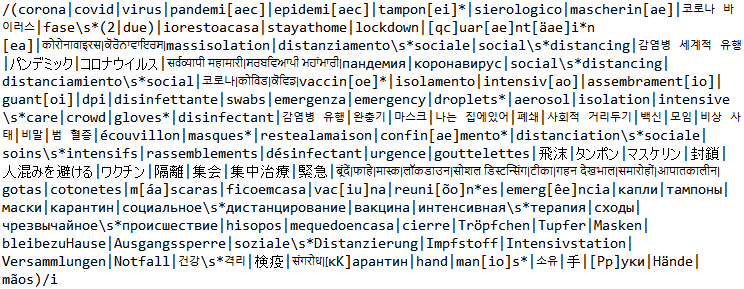
\includegraphics[width=0.95\linewidth]{pics/er.png}
	\end{figure}

	Come è possibile vedere, si è cercato di includere tutte le parole relative alla pandemia, e la loro traduzione nelle lingue di tutti i paesi che abbiamo considerato.
	
	L'espressione regolare è stata applicata sia ai titoli dei video, sia ai tags scelti per descrivere il video. Di seguito le query applicate:
	
	\begin{enumerate}
		\item Vengono create due nuove variabili che identificano se nel video sono presenti riferimenti al Covid-19 o meno, una per il titolo e una per i tags. Questa variabile viene inizializzata come \textit{false}:
		
			db.video\_merge.update(\{\},\{\$set : \{covid\_tags : false, covid\_title : false\}\},\{multi : true\})
		
		\item I video vengono analizzati singolarmente, e se l'espressione regolare (REGEX) restituisce un match positivo la variabile viene modificata in \textit{true}, prima per i tags:
		
			db.video\_merge.update(\{tags : \{\$in : [REGEX]\}\}, \{\$set : \{covid\_tags: true\}\}, \{multi : true\})
		
		\item Successivamente per il titolo:
		
			db.video\_merge.update(\{title : \{\$in : [REGEX]\}\}, \{\$set : \{covid\_title: true\}\}, \{multi : true\})
	\end{enumerate}
	L'applicazione delle query viene effettuata dallo script \textit{query\_covid.py}.
	
\subsection*{Scalabilità dell'algoritmo}

Una delle V su cui è stata posta la nostra attenzione è la Volume, ovvero come trattare e gestire grandi quantità di dati. 
In particolare abbiamo gestito:
\begin{itemize}
	\item prima sessione di scraping: 1.91 Gb
	\item seconda sessione di scraping: 1.11 Gb
	\item dati covid: 10 Mb
\end{itemize}
Per un totale di circa 3 Gb

Abbiamo deciso di utilizzare per trattare i dati con MongoDB, pertanto abbiamo implementato lo \textbf{Sharding}.
Sono stati costruiti tre shard, tutti in modalità replica set per garantire ridondanza in caso di guasti e frammentazione per rendere le query più efficienti nel momento in cui si andava a interrogare il \textit{router mongos}. I \textit{config server} sono stati anch'essi configurati come replica set. Come chiave di sharding è stata scelta il campo \textbf{country\_name}, perché le query per rispondere alle nostre domande vengono fatte sul singolo paese. Questo approccio è stato pensato anche nell'ottica di dividere la grande mole di dati in server disposti in ciascun paese. 

Per il dettaglio dei file di configurazione e altro vedere cartella \textit{sharding}.

Lo schema logico applicato è il seguente:
\begin{figure}[H]
	\centering
	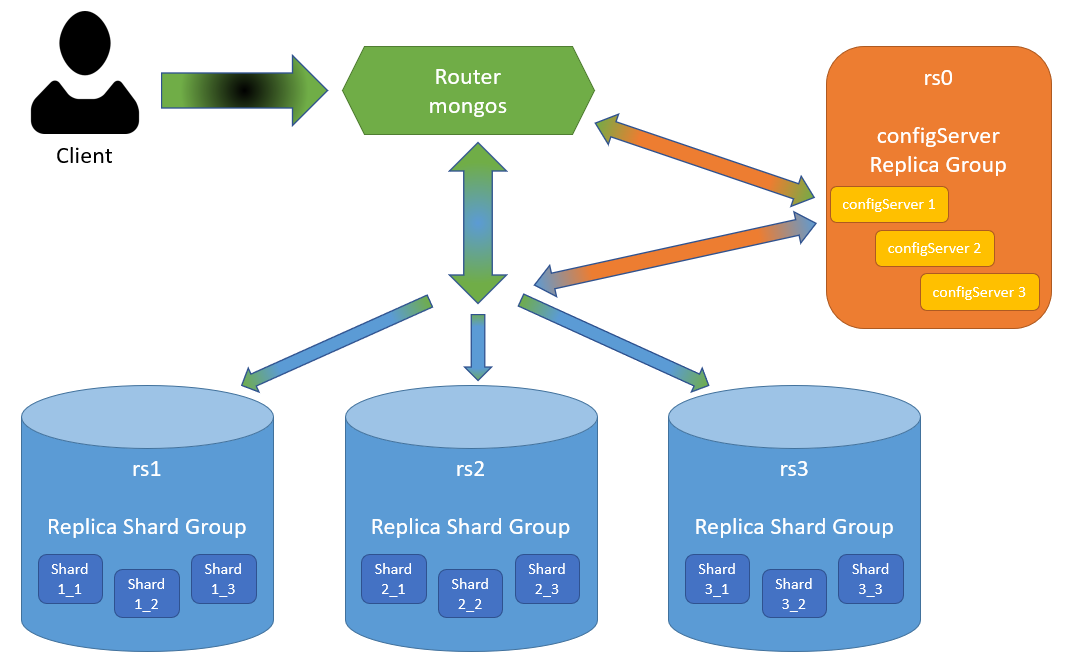
\includegraphics[width=0.8\linewidth]{pics/sharding.png}
	\caption{Pipeline sharding}
\end{figure}

In definitiva viene creato un database mongo chiamato \textit{YT\_data} con due collection: 
\begin{itemize}
	\item \textit{video\_all}: contiene tutti dati relativi alle due sessioni di presa dati
	\item \textit{video\_covid}: contiene i dati relativi alla seconda presa dati integrati con quelli relativi al covid
\end{itemize}

\subsection*{Query}
	Abbiamo eseguito alcune query per testare il funzionamento del database con e senza sharding, contenute negli script presenti nella cartella \textit{query}. In particolare si nota come la query 4, 5, 6 presentino dei risultati interessanti.
	
	In particolare:
	\begin{itemize}
		\item \textit{query 4}: elenco video a tema covid della categoria intrattenimento d'Italia
		\item \textit{query 5}: elenco video a tema covid della categoria intrattenimento e musica in Russia
		\item \textit{query 6}: elenco video a tema covid della categoria news \& politics in Italia e Germania
	\end{itemize}
	
	Per quanto riguarda tempo di esecuzione in millisecondi(\textit{executionTimeMillis}):
	\begin{table}[H]
		\centering
		\begin{tabular}{c|c|c}
			\textbf{Query} & \textbf{No Sharding} & \textbf{Sharding} \\
			\hline
			Query 4 & 635 & 126 \\
			Query 5 & 802 & 199 \\
			Query 6 & 1119 & 538 
		\end{tabular}
		\caption{differenze tempi in millisecondi}
	\end{table}
	
	Riguardo al numero di documenti esplorati per ottenere la risposta:
	\begin{table}[H]
		\centering
		\begin{tabular}{c|c|c}
			\textbf{Query} & \textbf{No Sharding} & \textbf{Sharding} \\
			\hline
			Query 4 & 444207 & 36950 \\
			Query 5 & 444207 & 28715 \\
			Query 6 & 444207 & 444207 
		\end{tabular}
		\caption{differenze numero di documenti esplorati}
	\end{table}
	
	Si può notare come per la query 4 e 5 vengono esplorati un numero di video molto inferiori nel database con sharding rispetto a quello senza, questo si traduce in un miglioramento dei tempi di esecuzione. La query 6, poiché necessità di informazioni riguardanti tutti i paesi, esplora tutti i dati a prescindere degli shard, quindi non ha alcun miglioramento prestazionale.
	
	Per il dettaglio vedere i file di risposta nella cartella \textit{query}.
%Per farlo ci occupiamo di effettuare la nostra analisi su partizionamenti sempre maggiori del nostro dataset e registriamo il tempo di esecuzione del nostro programma, effettuiamo poi una semplice regressione per vedere di che tipo di crescita stiamo parlando, ovviamente più la crescita è minore più il nostro algoritmo scala bene per volumi di dati maggiori. Presentiamo di seguito la registrazione dei tempi rispetto al partizionamento dei dati. 

%\begin{figure}[H]
%	\centering
%	\includegraphics[height=0.3 \linewidth]{pict/times.png}
%	\caption{Crescita del tempo di esecuzione rispetto all'aumentare del partizionamento.}
%\end{figure}

\section*{Visualizzazione}

La scelta delle visualizzazioni è stata guidata dalle domande di ricerca che ci siamo posti: 
\begin{itemize}
	\item Come variano le tipologie dei video in tendenza dal periodo precedente al coronavirus alla quarantena?
	\item È vero che la fruizione di video su Youtube riguardanti il Covid-19 segue l'andamento dei dati sull'epidemia?
\end{itemize}

\subsection*{Scelta features}
Per rispondere in modo coerente alle nostre domande di ricerca abbiamo deciso di concentrarci sulle seguenti features del nostro dataset.
\begin{itemize}
	\item View Count
	\item Covid Title
	\item Covid Tags
	\item Trending Date
	\item Title
	\item Cases New
\end{itemize}

\subsection*{Scelta della visualizzazione}

Abbiamo utilizzato due infografiche diverse per le domande di ricerca, poiché ci è sembrata incompatibile un'unica visualizzazione per entrambe.


\paragraph{Prima infografica} La prima infografica consiste nella combinazione di due diverse visualizzazioni:
\begin{itemize}
	\item Un lollipop chart temporale che rappresenta il numero video entrato in tendenza ogni giorno. Sottolineamo che l'asse orizzontale rappresente le date di dicembre-gennaio e di marzo-maggio, in accordo con la nostra raccolta dati.
	\item Un bubble chart, dove ogni bolla è un video, la sua grandezza rappresenta il numero di visualizzazioni e il colore la categoria di appartenenza.
\end{itemize}

La combinazione di queste due visualizzazioni permette di capire se il contenuto dei video entrati in tendenza nel periodo precedente al Covid-19 e  durante la quarantena differiscano significativamente. Per farlo è sufficiente selezionare due giorni contemporaneamente e vedere il cambiamento nelle bolle. L'esplorazione di questa infografica avviene per passi guidati attraverso una storia, in modo da introdurre all'utente tutte le informazioni che questa visualizzazione può offrire. Di seguito una visione sommaria dell'infografica comprensiva dei contesti:
\begin{figure}[H]
	\centering
	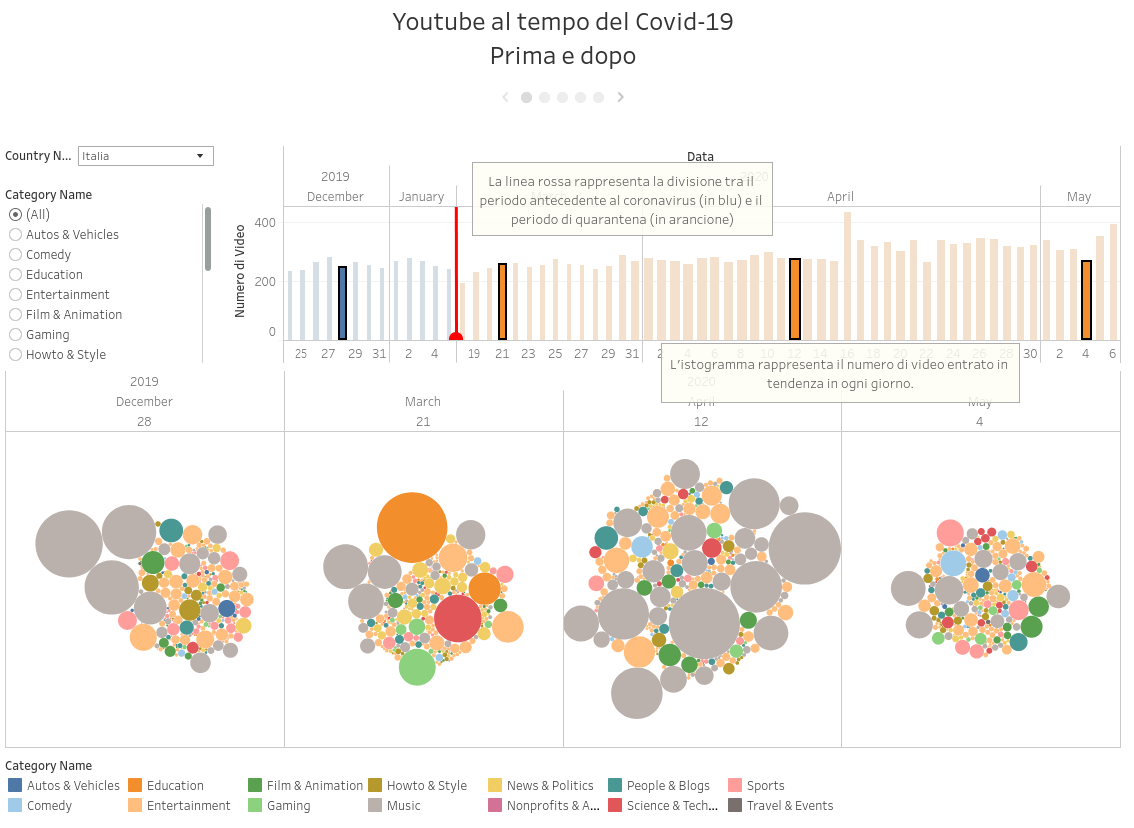
\includegraphics[height=0.5 \linewidth]{pics/prima_infografica.png}
	\caption{Prima infografica.}
\end{figure}

\paragraph{Seconda infografica} Per quanto riguarda la risposta alla seconda domanda di ricerca abbiamo deciso di utilizzare una infografica composta da due visualizzazioni come precedentemente. In particolare:
\begin{itemize}
	\item Un misto tra un bar chart e un line chart temporale. In questa visualizzazione abbiamo fatto risaltare la differenza percentuale tra una rilevazione e quella del giorno precedente. Il line chart riguarda l'aumento percentuale del numero di video in tendenza relativi al Covid-19 mentre il bar chart riguarda l'aumento percentuale dei nuovi casi di Covid-19 rispetto al giorno precedente. 
	Abbiamo utilizzato questo tipo di grafico in modo da poter vedere se le notizie negative o positive dei dati riguardanti il Covid-19 abbia influito sulla fruizione online dei video concernenti lo stesso argomento.
	L'utilizzo di un bar chart e un line chart è dovuto al fatto che dai questionari è risultata più apprezzata questa scelta per riconoscere le due variabili.

	\item Uno stacked bar chart che rappresenta il numero di video per categoria che riguardano il Covid-19. La visualizzazione può essere filtrata per giorno semplicemente interagendo con la prima visualizzazione.
\end{itemize}

La combinazione di queste due visualizzazioni consente di rispondere alla seconda domanda di ricerca che ci siamo posti precedentemente. Proponiamo di seguito una visione sommaria dell'infografica comprensiva dei contesti.

\begin{figure}[H]
	\centering
	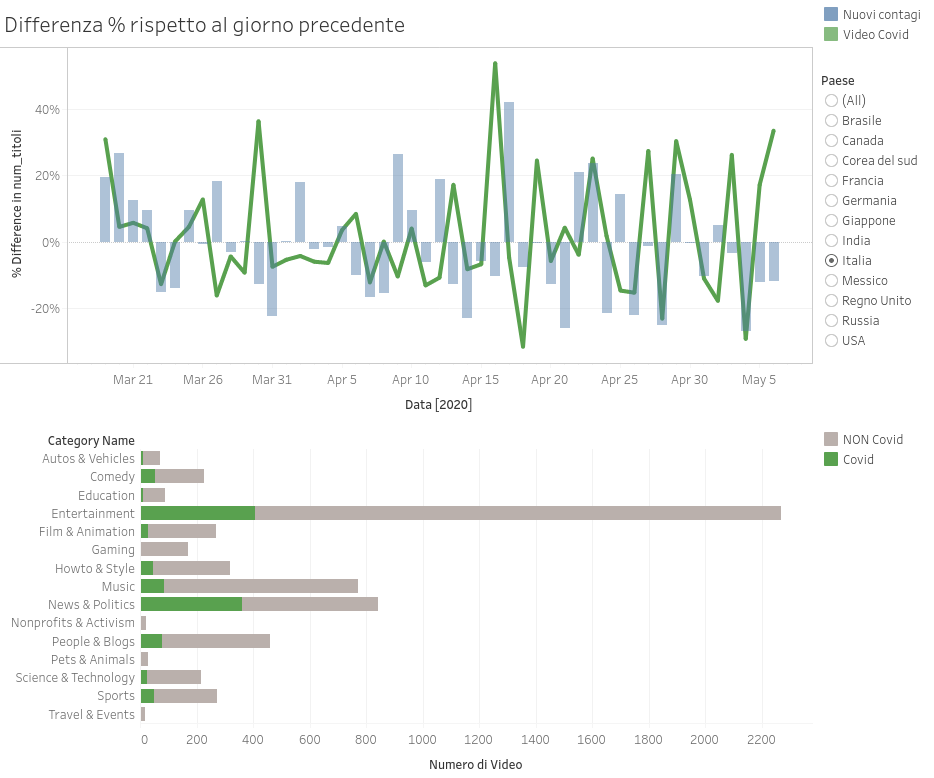
\includegraphics[height=0.5 \linewidth]{pics/seconda_infografica.png}
	\caption{Seconda infografica.}
\end{figure}
\subsection*{Valutazione della qualità}
La valutazione della qualità si è articolata in tre passaggi:

\paragraph{User Test} Durante questa fase ci siamo occupati di sottoporre la nostra infografica a sei persone lasciando completa libertà di esplorazione. Le varie interazioni sono state registrate in modo da far sì che potessero emergere le diverse problematiche di cui non ci siamo accorti in fase di realizzazione delle infografiche. Esponiamo le problematiche emerse durante questa fase di valutazione e le correzioni applicate:

\begin{itemize}
	\item \textit{Problema 1:} Il fatto di avere due variabili sotto forma di linea nella prima infografica rende difficoltoso distinguerle nonostante il colore.\\\textit{Soluzione 1:} Abbiamo deciso di assegnare ad una variabile la forma "linea" e all'altra variabile la forma "barra".
	\item  \textit{Problema 2: Come comprendere che cliccare sul bianco significa non avere nessun giorno selezionato, e quindi una visione complessiva.}\\\textit{Soluzione 2: Introdurre l'infografica mediante storie che possano guidare l'utente nell'esplorazione.} 
	\item  \textit{Problema 3: Come comprendere quali video sono nella categoria Covid e quali no.} \\\textit{Soluzione 3: Una legenda semplificata e l'utilizzo di bar chart sovrapposti di colori diversi.} 
\end{itemize}
\paragraph{Risultati dei task} Durante questa fase ci siamo occupati di sottoporre tre diverse richieste per ogni infografica a 24 utenti; questi task devono essere soddisfatti esplorando in maniera interattiva. I task da risolvere sono stati i seguenti:
\begin{enumerate}
	\item Per la \textit{prima infografica:}
	\begin{itemize}
		\item Nella giornata del 20 marzo quale video ha avuto più visualizzazioni e a quale categoria appartiene?  \textit{Science \& technology, IPad Pro}
		\item Della categoria Entertainment quali sono i canali che hanno fatto più visualizzazioni a Natale e a Pasqua? \textit{The Late Show with Corbin, Mr Beast}
		\item Nella categoria sport confronta il 30 dicembre e 10 aprile in Germania. Qual è il titolo dei video più visti per ciascun giorno?\\
		\textit{Sampdoria 1-2 Juventus | Ronaldo Header Winds it for the Visitors | Serie A TIM \\ F1 Esports Virtual Grand Prix Highlights | Aramco}
	\end{itemize}
	\item Per la \textit{seconda infografica:}
\begin{itemize}
	\item Trova la categoria che ha avuto più video Covid-19 il giorno 27 Marzo in Italia? \textit{News and Politics}
	\item Quanti video Covid-19 della categoria "People and Blogs" ci sono stati negli USA? \textit{12}
	\item Quanti nuovi contagi ha avuto la Corea del Sud il 12 Aprile? \textit{62}
\end{itemize}
\end{enumerate}

Sono stati registrati i tempi in cui gli utenti riuscivano a completare questi obiettivi e sono stati visualizzati i risultati nei seguenti box plot:
%\begin{figure}[H]
%	\centering
%	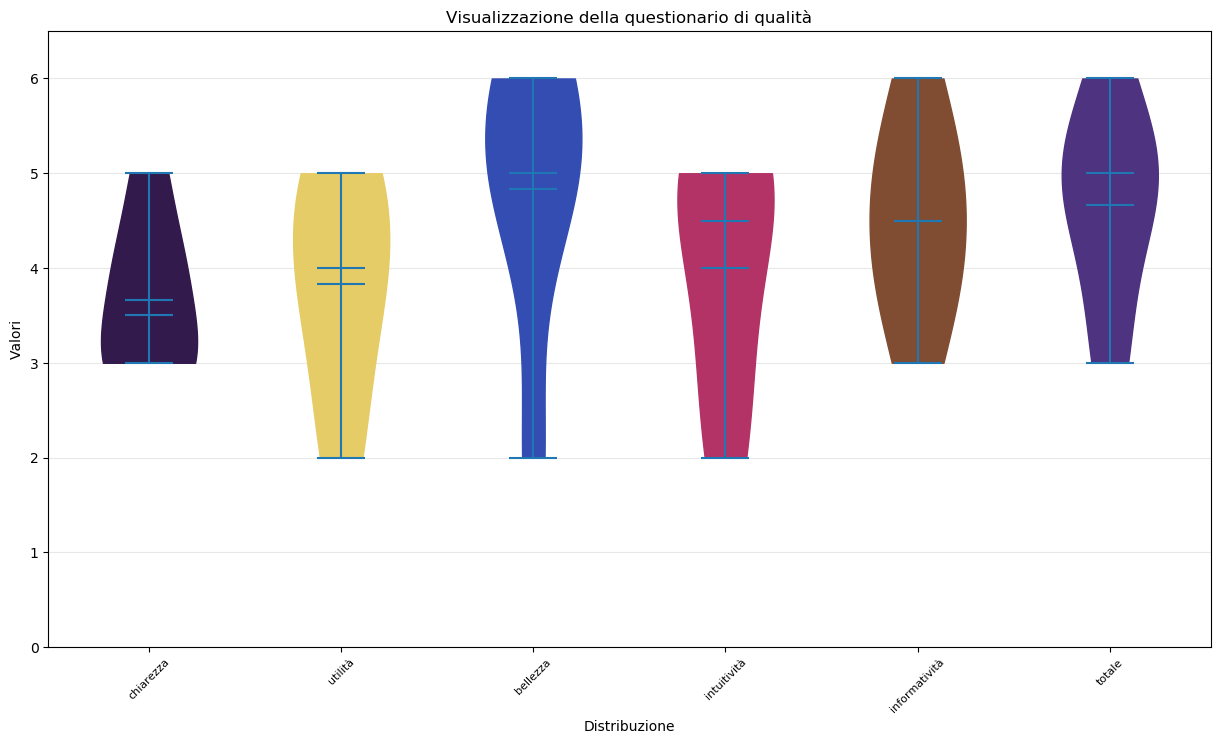
\includegraphics[height=0.3 \linewidth]{pict/violin_plot.png}
%	\caption{Tempi di completamento dei task.}
%\end{figure}
Questa visualizzazione è utile per capire se le nostre infografiche sono troppo dispersive oppure se riescono a essere facili e intuitive.

\paragraph{Questionari} Per quanto riguarda l'ultima fase è stato somministrato un questionario di valutazione della qualità a 24 persone articolato nella seguente maniera:
\begin{itemize}
	\item Come valuti la chiarezza dell' infografica?
	\item Come valuti l'utilità dell'infografica?
	\item Quanto valuti la bellezza dell'infografica?
	\item Come valuti l'intuitività dell'infografica?
	\item Quanto è stata informativa l'infografica?
	\item Come valuti complessivamente l'infografica?
\end{itemize}
Le risposte sono state registrate grazie al tool "Questionari di Google". Una volta registrati i risultati è stata controllata che la valutazione dell'infografica fosse coerente con una ricostruzione complessiva della regressione con i coefficienti di Cabitza-Locoro.
%\begin{figure}[H]
%	\centering
%	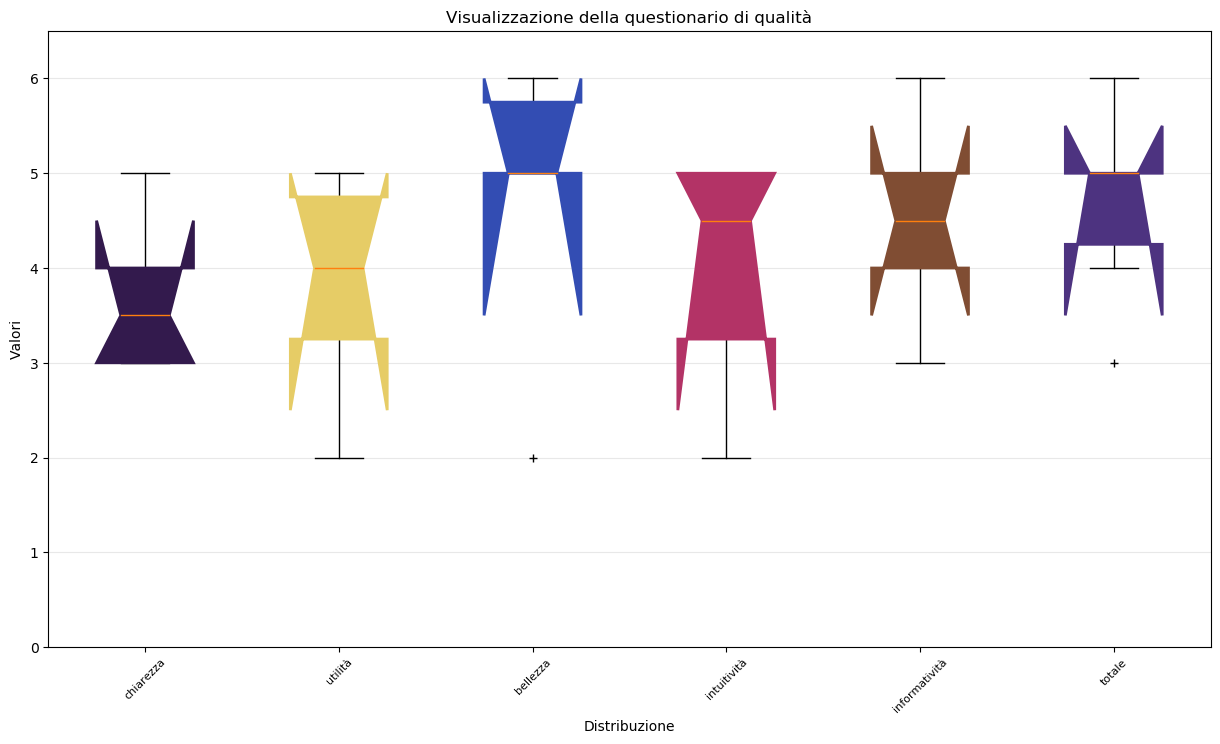
\includegraphics[height=0.3 \linewidth]{pict/box_plot.png}
%	\caption{Dispersione delle risposte del questionario.}
%\end{figure}
L'utilizzo di un box plot è risultato molto comodo per la registrazione delle risposte poiché la media è un indicatore di tendenza centrale e non fornisce alcuna informazione sulla distribuzione di questi dati.
Per quanto riguarda invece la coerenza della valutazione rispetto alla ricostruzione data dai coefficienti abbiamo avuto la seguente distribuzione:
%\begin{figure}[H]
%	\centering
%	\includegraphics[height=0.3 \linewidth]{pict/regressione.png}
%	\caption{$R^{2} = 0.75$.}
%\end{figure}

\section*{Conclusioni e prospettive future}
In conclusione possiamo affermare che vi sono rilevanti differenze nelle tendenze di Youtube tra prima e durante l'epidemia di Covid-19. 

La prima infografica mostra come la distribuzione dei video nelle varie categorie sia cambiata. Ad esempio per quanto riguarda l'Italia la categoria di Sport subisce una drastica diminuzione, presumibilmente dovuta al blocco di tutti gli sport durante il lockdown; così come la categoria News \& politics trova una più alta presenza nel periodo covid rispetto al periodo precedente.

La seconda infografica mostra che la variazione giornaliera del numero di contagi non influenza strettamente il numero di contenuti nelle tendenze legati al Covid. In alcuni frangenti si nota una certa relazione tra le due misure, ad esempio in Italia nel periodo di fine marzo, inizio aprile. Ne consegue che probabilmente l'impatto dei numeri ufficiali relativi ai contagi non abbiano influenzato in modo significativo le tendenze giornaliere di youtube.

Da queste due infografiche possiamo concludere che i gusti degli utenti di youtube hanno subito un evidente cambiamento durante il periodo dell'epidemia, questo cambiamento è avvenuto gradualmente e non strettamente legato ai numeri ufficiali dei contagi.

\paragraph{Prospettive future}Possibile regressione e vedere cosa succede dopo che le acque si sono calmate 



\end{document}